\documentclass[10pt,a4paper]{article}
\usepackage[T1]{fontenc}
\usepackage[utf8]{inputenc}
\IfFileExists{lmodern.sty}{\usepackage{lmodern}}{}
\usepackage[margin=18mm,headheight=14pt]{geometry}
\usepackage[table]{xcolor}
\usepackage{graphicx}
\usepackage{booktabs}
\usepackage{longtable}
\usepackage{array}
\usepackage{amssymb}
\usepackage{fancyhdr}
\IfFileExists{lastpage.sty}{\usepackage{lastpage}\newcommand{\ofpages}{\ of \pageref{LastPage}}}{\newcommand{\ofpages}{}}
\IfFileExists{caption.sty}{\usepackage{caption}\captionsetup{font=small,labelfont={bf,color=navy}}}{}
\IfFileExists{enumitem.sty}{\usepackage{enumitem}\setlist[itemize]{leftmargin=14pt,itemsep=2pt,topsep=2pt}}{}
\usepackage[hidelinks]{hyperref}
\definecolor{navy}{HTML}{16324F}
\definecolor{accent}{HTML}{2A6FDB}
\definecolor{zebra}{HTML}{F4F6F9}
\definecolor{noteinfo}{HTML}{EEF4FD}
\definecolor{notewarn}{HTML}{FFF6E5}
\definecolor{muted}{HTML}{6B7685}
\setlength{\parindent}{0pt}
\setlength{\parskip}{4pt}
\renewcommand{\arraystretch}{1.15}
\pagestyle{fancy}\fancyhf{}
\renewcommand{\headrulewidth}{0.3pt}
\fancyfoot[L]{\color{muted}\footnotesize Generated by croco\_bench.py}
\fancyfoot[R]{\color{muted}\footnotesize Page \thepage\ofpages}
\fancyhead[L]{\color{muted}\footnotesize CROCO Benchmark Report $\cdot$ REGIONAL $\triangleright$ BENGUELA\_LR  $\cdot$  grid 60 $\times$ 40 $\times$ 32  $\cdot$  30 days per run  $\cdot$  2026-10-24 17:35}
\begin{document}
\noindent\colorbox{navy}{\parbox{\dimexpr\linewidth-2\fboxsep}{\vspace{8pt}
{\color{white}\LARGE\bfseries CROCO Benchmark Report}\\[4pt]
{\color{white!80!accent}\small REGIONAL $\triangleright$ BENGUELA\_LR  $\cdot$  grid 60 $\times$ 40 $\times$ 32  $\cdot$  30 days per run  $\cdot$  2026-10-24 17:35}\vspace{6pt}}}
\par\noindent{\color{accent}\rule{\linewidth}{2pt}}\par\medskip
{\small\noindent\begin{tabular}{@{}p{0.24\linewidth}p{0.73\linewidth}@{}}
\textbf{\textcolor{navy}{Configuration}} & \texttt{cppdefs.h} block \texttt{REGIONAL}, case \texttt{BENGUELA\_LR} \\[1pt]
\textbf{\textcolor{navy}{Grid (param.h)}} & LLm $\times$ MMm $\times$ N = \textbf{60 $\times$ 40 $\times$ 32} (active branch \texttt{REGIONAL $\triangleright$ BENGUELA\_LR}, line 10) \\[1pt]
\textbf{\textcolor{navy}{Machine}} & \texttt{vm}: Intel(R) Xeon(R) Processor @ 2.10GHz; 2 physical / 2 logical CPUs \\[1pt]
\textbf{\textcolor{navy}{Cores used}} & 16 (CPU 0-15), up to 16 simultaneous runs \\[1pt]
\textbf{\textcolor{navy}{Run directory}} & \texttt{/home/claude/mock/case} \\[1pt]
\textbf{\textcolor{navy}{Simulated period}} & 30 days per run; original croco.in dt = 3600 s, NDTFAST = 60 (\texttt{fixed}) \\[1pt]
\end{tabular}}\par\medskip
\section{Key results}
\begin{center}\small\rowcolors{1}{zebra}{zebra}
\begin{tabular}{!{\color{accent}\vrule width 2pt}>{\raggedright\arraybackslash}p{0.29\linewidth}!{\color{accent}\vrule width 2pt}>{\raggedright\arraybackslash}p{0.29\linewidth}!{\color{accent}\vrule width 2pt}>{\raggedright\arraybackslash}p{0.29\linewidth}}
{\scriptsize\color{muted}RECOMMENDED DT}\newline{\large\bfseries\color{navy} 1200 s}\newline{\scriptsize 3600 / 3 steps per hour; largest stable 1790 s} & {\scriptsize\color{muted}RECOMMENDED CORES $\cdot$ MPI}\newline{\large\bfseries\color{navy} 8 cores}\newline{\scriptsize layout 4x2, E = 0.506} & {\scriptsize\color{muted}RECOMMENDED CORES $\cdot$ OPENMP}\newline{\large\bfseries\color{navy} 4 cores}\newline{\scriptsize layout 1x4, E = 0.581} \\[3pt]
{\scriptsize\color{muted}FASTEST RUN}\newline{\large\bfseries\color{navy} MPI 12 cores}\newline{\scriptsize 6 $\times$ 2, 1.5 s per 30 days} & {\scriptsize\color{muted}BAROTROPIC CFL AT RECOMMENDED DT}\newline{\large\bfseries\color{navy} 0.567}\newline{\scriptsize advective 0.414; first BLOW UP at 1800 s} & {\scriptsize\color{muted}SERIAL REFERENCE T(1)}\newline{\large\bfseries\color{navy} 7.4 s}\newline{\scriptsize 1 core, no OpenMP/MPI, dt = 1200 s} \\[3pt]
\end{tabular}\end{center}
\begin{itemize}
\item \textbf{Recommended time step: 1200 s} = 3600 / 3, the largest integer dt that divides 3600 without exceeding the largest stable dt. All times and efficiencies in this report were measured with it.
\item \textbf{Largest stable dt found:} 1790 s (NDTFAST = 60, barotropic dt = 29.83 s).
\item \textbf{Stability limit} between 1790 s (stable) and 1800 s (first BLOW UP).
\item \textbf{MPI:} up to \textbf{8 cores} (layout 4x2, efficiency 0.506 > 0.5).
\item \textbf{OPENMP:} up to \textbf{4 cores} (layout 1x4, efficiency 0.581 > 0.5).
\item \textbf{Fastest configuration:} MPI with 12 cores, layout 6 $\times$ 2 (NP\_XI $\times$ NP\_ETA), 1.5 s per 30 days (71760.8 simulated days per wall-clock hour), measured alone on the machine.
\end{itemize}
\section{Time-step search (serial run)}
All runs of this stage use the serial build (1 core, \texttt{OPENMP} and \texttt{MPI} undefined). Starting from the reference dt (600 s), dt is doubled while the run is stable; after the first BLOW UP the next dt is the midpoint between the last stable dt and the last BLOW UP, and the search stops after two BLOW UPs in a row. Rules: a dt larger than one that blew up is never tested, and when going down the search never goes below a stable dt whose half is also stable.

{\footnotesize\rowcolors{2}{white}{zebra}
\begin{longtable}{rlrl}
\caption{Decision sequence of the time-step search.}\\
\toprule
\textbf{Step} & \textbf{Phase} & \textbf{dt [s]} & \textbf{Result} \\
\midrule
\endfirsthead
\toprule
\textbf{Step} & \textbf{Phase} & \textbf{dt [s]} & \textbf{Result} \\
\midrule
\endhead
\bottomrule
\endfoot
1 & up & 600 & stable \\
2 & up & 1200 & stable \\
3 & up & 2400 & BLOW UP \\
4 & bisect & 1800 & BLOW UP \\
5 & bisect & 1500 & stable \\
6 & bisect & 1650 & stable \\
7 & bisect & 1725 & stable \\
8 & bisect & 1762 & stable \\
9 & bisect & 1781 & stable \\
10 & bisect & 1790 & stable \\
\end{longtable}}
{\footnotesize\rowcolors{2}{white}{zebra}
\begin{longtable}{rrrlrrrr}
\caption{Stability and Courant numbers for every dt tested ($\star$ = recommended dt). Internal-wave CFL estimated with an assumed c$_1$ = 2.0 m/s.}\\
\toprule
\textbf{dt [s]} & \textbf{NDTFAST} & \textbf{dt\_fast [s]} & \textbf{Status} & \textbf{CFL barotropic} & \textbf{CFL internal} & \textbf{CFL advective} & \textbf{Best time} \\
\midrule
\endfirsthead
\toprule
\textbf{dt [s]} & \textbf{NDTFAST} & \textbf{dt\_fast [s]} & \textbf{Status} & \textbf{CFL barotropic} & \textbf{CFL internal} & \textbf{CFL advective} & \textbf{Best time} \\
\midrule
\endhead
\bottomrule
\endfoot
600 & 60 & 10.00 & OK & 0.284 & 0.768 & 0.207 & 14.6 s \\
1200 $\star$ & 60 & 20.00 & OK & 0.567 & 1.537 & 0.414 & 1.5 s \\
1500 & 60 & 25.00 & OK & 0.709 & 1.921 & 0.517 & 6.1 s \\
1650 & 60 & 27.50 & OK & 0.780 & 2.113 & 0.569 & 5.6 s \\
1725 & 60 & 28.75 & OK & 0.815 & 2.209 & 0.595 & 5.7 s \\
1762 & 60 & 29.37 & OK & 0.833 & 2.256 & 0.608 & 5.6 s \\
1781 & 60 & 29.68 & OK & 0.842 & 2.281 & 0.614 & 5.7 s \\
1790 & 60 & 29.83 & OK & 0.846 & 2.292 & 0.618 & 5.8 s \\
1800 & 60 & 30.00 & BLOWUP & 0.851 & 2.305 & 0.621 & -- \\
2400 & 60 & 40.00 & BLOWUP & 1.134 & 3.074 & 0.828 & -- \\
\end{longtable}}
\begin{figure}[htbp]\centering
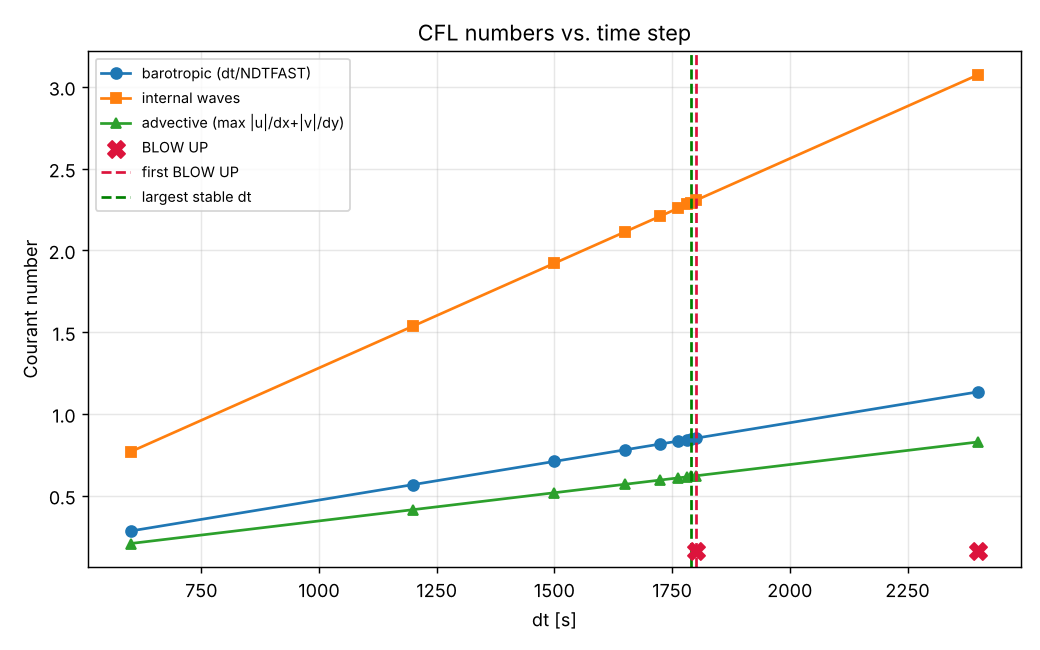
\includegraphics[width=\linewidth,height=0.55\textheight,keepaspectratio]{cfl_vs_dt.png}
\caption{Courant numbers versus time step; the dashed lines mark the largest stable dt and the first BLOW UP.}
\end{figure}
\section{Core-count exploration}
OpenMP and MPI start at 12 cores. For each core count every valid nx $\times$ ny decomposition is run and the fastest is kept. With E(n) = T(1) / (n $\cdot$ T(n)): if E > 0.5 the next test uses 2 more cores, otherwise 2 fewer; each mode stops when the direction reverses or the core limit is reached.

{\footnotesize\rowcolors{2}{white}{zebra}
\begin{longtable}{rcrrl}
\caption{OPENMP exploration path (stop: direction reversed at 4 cores).}\\
\toprule
\textbf{Cores} & \textbf{Best layout} & \textbf{Time} & \textbf{Efficiency E} & \textbf{Decision} \\
\midrule
\endfirsthead
\toprule
\textbf{Cores} & \textbf{Best layout} & \textbf{Time} & \textbf{Efficiency E} & \textbf{Decision} \\
\midrule
\endhead
\bottomrule
\endfoot
12 & 4x3 & 1.9 s & 0.329 & E $\leq$ 0.5 $\rightarrow$ $-$2 \\
10 & 5x2 & 2.0 s & 0.362 & E $\leq$ 0.5 $\rightarrow$ $-$2 \\
8 & 4x2 & 2.2 s & 0.421 & E $\leq$ 0.5 $\rightarrow$ $-$2 \\
6 & 2x3 & 2.5 s & 0.493 & E $\leq$ 0.5 $\rightarrow$ $-$2 \\
4 & 1x4 & 3.2 s & 0.581 & E > 0.5 $\rightarrow$ +2 \\
\end{longtable}}
{\footnotesize\rowcolors{2}{white}{zebra}
\begin{longtable}{rcrrl}
\caption{MPI exploration path (stop: direction reversed at 8 cores).}\\
\toprule
\textbf{Cores} & \textbf{Best layout} & \textbf{Time} & \textbf{Efficiency E} & \textbf{Decision} \\
\midrule
\endfirsthead
\toprule
\textbf{Cores} & \textbf{Best layout} & \textbf{Time} & \textbf{Efficiency E} & \textbf{Decision} \\
\midrule
\endhead
\bottomrule
\endfoot
12 & 6x2 & 1.5 s & 0.409 & E $\leq$ 0.5 $\rightarrow$ $-$2 \\
10 & 5x2 & 1.7 s & 0.444 & E $\leq$ 0.5 $\rightarrow$ $-$2 \\
8 & 4x2 & 1.8 s & 0.506 & E > 0.5 $\rightarrow$ +2 \\
\end{longtable}}
\begin{figure}[htbp]\centering
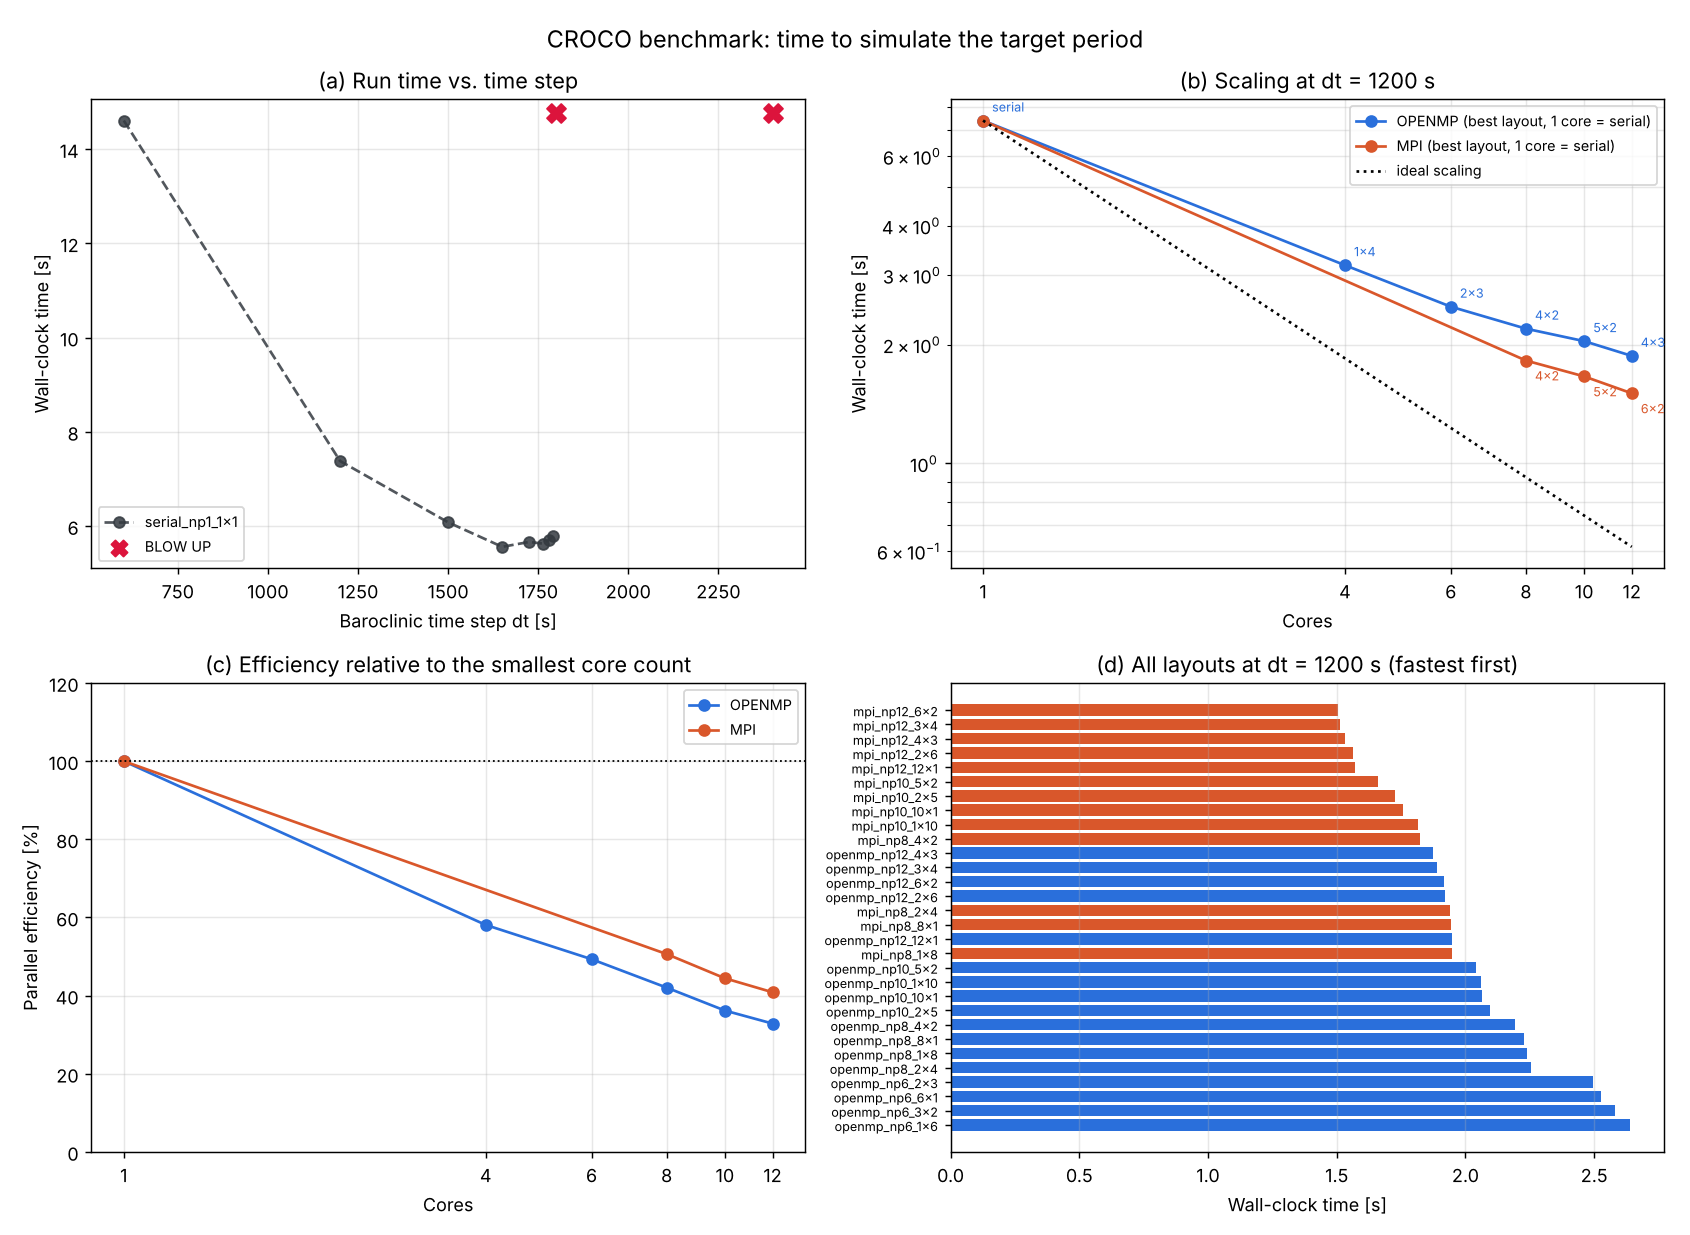
\includegraphics[width=\linewidth,height=0.55\textheight,keepaspectratio]{benchmark_summary.png}
\caption{(a) run time versus dt, (b) scaling and (c) parallel efficiency at dt = 1200 s, (d) every layout tested.}
\end{figure}
\section{Efficiency study (NLHPC format)}
Format of the \href{https://wiki.nlhpc.cl/Estudio_de_Eficiencia}{NLHPC efficiency study}, at dt = 1200 s and 30 days simulated, with the best layout of each core count: \textbf{speed-up} S(n) = T(1) / T(n), \textbf{efficiency} E(n) = S(n) / n. T(1) is the serial run (1 core, built without OpenMP or MPI). Recommended: the largest core count with E > 0.5.

{\footnotesize\rowcolors{2}{white}{zebra}
\begin{longtable}{lrrrr}
\caption{MPI: recommended \textbf{8 cores}.}\\
\toprule
\textbf{No. of cores} & \textbf{1} & \textbf{8} & \textbf{10} & \textbf{12} \\
\midrule
\endfirsthead
\toprule
\textbf{No. of cores} & \textbf{1} & \textbf{8} & \textbf{10} & \textbf{12} \\
\midrule
\endhead
\bottomrule
\endfoot
Layout & serial & 4x2 & 5x2 & 6x2 \\
Time [s] & 7.38 & 1.82 & 1.66 & 1.50 \\
Speed-up & 1.00 & 4.05 & 4.44 & 4.90 \\
Efficiency & \textbf{1.00} & \textbf{0.51} & 0.44 & 0.41 \\
Measured alone & yes & yes & yes & yes \\
\end{longtable}}
{\footnotesize\rowcolors{2}{white}{zebra}
\begin{longtable}{lrrrrrr}
\caption{OPENMP: recommended \textbf{4 cores}.}\\
\toprule
\textbf{No. of cores} & \textbf{1} & \textbf{4} & \textbf{6} & \textbf{8} & \textbf{10} & \textbf{12} \\
\midrule
\endfirsthead
\toprule
\textbf{No. of cores} & \textbf{1} & \textbf{4} & \textbf{6} & \textbf{8} & \textbf{10} & \textbf{12} \\
\midrule
\endhead
\bottomrule
\endfoot
Layout & serial & 1x4 & 2x3 & 4x2 & 5x2 & 4x3 \\
Time [s] & 7.38 & 3.18 & 2.49 & 2.19 & 2.04 & 1.87 \\
Speed-up & 1.00 & 2.32 & 2.96 & 3.36 & 3.62 & 3.94 \\
Efficiency & \textbf{1.00} & \textbf{0.58} & 0.49 & 0.42 & 0.36 & 0.33 \\
Measured alone & yes & yes & yes & yes & yes & yes \\
\end{longtable}}
\begin{figure}[htbp]\centering
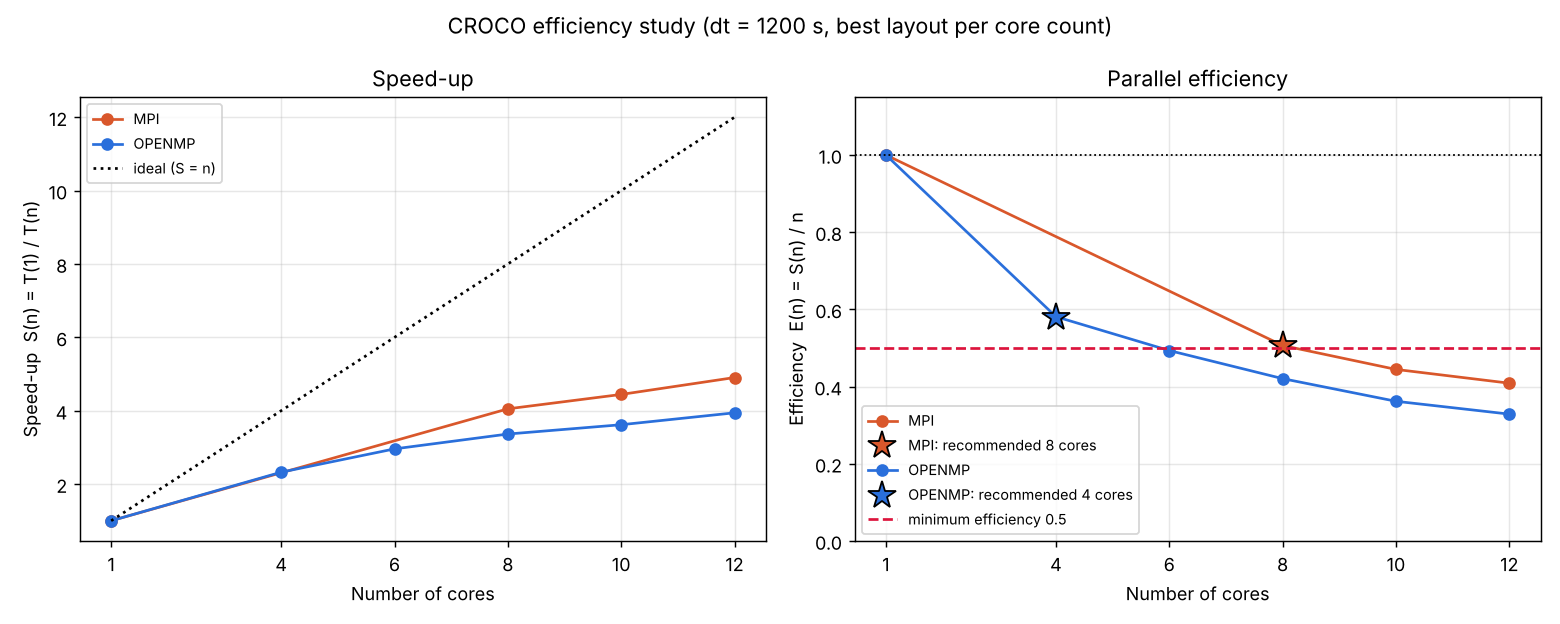
\includegraphics[width=\linewidth,height=0.55\textheight,keepaspectratio]{efficiency_study.png}
\caption{Speed-up (left, with the ideal line) and parallel efficiency (right, with the threshold); stars mark the recommended core count of each mode.}
\end{figure}
\section{All layouts at dt = 1200 s}
{\scriptsize\rowcolors{2}{white}{zebra}
\begin{longtable}{lrcrrrrlp{0.16\linewidth}}
\caption{Every layout at dt = 1200 s, fastest first; speed-up and efficiency relative to the fastest run with 1 core(s).}\\
\toprule
\textbf{Mode} & \textbf{Cores} & \textbf{Layout} & \textbf{Time} & \textbf{Days/hour} & \textbf{Speed-up} & \textbf{Efficiency} & \textbf{Measured} & \textbf{Status} \\
\midrule
\endfirsthead
\toprule
\textbf{Mode} & \textbf{Cores} & \textbf{Layout} & \textbf{Time} & \textbf{Days/hour} & \textbf{Speed-up} & \textbf{Efficiency} & \textbf{Measured} & \textbf{Status} \\
\midrule
\endhead
\bottomrule
\endfoot
MPI & 12 & 6 $\times$ 2 & 1.5 s & 71760.8 & 4.90 & 41 \% & alone & OK \\
MPI & 12 & 3 $\times$ 4 & 1.5 s & 71475.8 & 4.88 & 41 \% & alone & OK \\
MPI & 12 & 4 $\times$ 3 & 1.5 s & 70404.2 & 4.81 & 40 \% & alone & OK \\
MPI & 12 & 2 $\times$ 6 & 1.6 s & 69053.7 & 4.72 & 39 \% & alone & OK \\
MPI & 12 & 12 $\times$ 1 & 1.6 s & 68746.0 & 4.70 & 39 \% & alone & OK \\
MPI & 10 & 5 $\times$ 2 & 1.7 s & 65021.1 & 4.44 & 44 \% & alone & OK \\
MPI & 10 & 2 $\times$ 5 & 1.7 s & 62500.0 & 4.27 & 43 \% & alone & OK \\
MPI & 10 & 10 $\times$ 1 & 1.8 s & 61503.4 & 4.20 & 42 \% & alone & OK \\
MPI & 10 & 1 $\times$ 10 & 1.8 s & 59536.9 & 4.07 & 41 \% & alone & OK \\
MPI & 8 & 4 $\times$ 2 & 1.8 s & 59275.5 & 4.05 & 51 \% & alone & OK \\
OPENMP & 12 & 4 $\times$ 3 & 1.9 s & 57692.3 & 3.94 & 33 \% & alone & OK \\
OPENMP & 12 & 3 $\times$ 4 & 1.9 s & 57142.9 & 3.91 & 33 \% & alone & OK \\
OPENMP & 12 & 6 $\times$ 2 & 1.9 s & 56367.4 & 3.85 & 32 \% & alone & OK \\
OPENMP & 12 & 2 $\times$ 6 & 1.9 s & 56220.7 & 3.84 & 32 \% & alone & OK \\
MPI & 8 & 2 $\times$ 4 & 1.9 s & 55698.8 & 3.81 & 48 \% & alone & OK \\
MPI & 8 & 8 $\times$ 1 & 1.9 s & 55527.0 & 3.79 & 47 \% & alone & OK \\
OPENMP & 12 & 12 $\times$ 1 & 1.9 s & 55498.5 & 3.79 & 32 \% & alone & OK \\
MPI & 8 & 1 $\times$ 8 & 1.9 s & 55498.5 & 3.79 & 47 \% & alone & OK \\
OPENMP & 10 & 5 $\times$ 2 & 2.0 s & 52941.2 & 3.62 & 36 \% & alone & OK \\
OPENMP & 10 & 1 $\times$ 10 & 2.1 s & 52427.2 & 3.58 & 36 \% & alone & OK \\
OPENMP & 10 & 10 $\times$ 1 & 2.1 s & 52350.9 & 3.58 & 36 \% & alone & OK \\
OPENMP & 10 & 2 $\times$ 5 & 2.1 s & 51502.1 & 3.52 & 35 \% & alone & OK \\
OPENMP & 8 & 4 $\times$ 2 & 2.2 s & 49225.2 & 3.36 & 42 \% & alone & OK \\
OPENMP & 8 & 8 $\times$ 1 & 2.2 s & 48474.0 & 3.31 & 41 \% & alone & OK \\
OPENMP & 8 & 1 $\times$ 8 & 2.2 s & 48214.3 & 3.30 & 41 \% & alone & OK \\
OPENMP & 8 & 2 $\times$ 4 & 2.3 s & 47893.6 & 3.27 & 41 \% & alone & OK \\
OPENMP & 6 & 2 $\times$ 3 & 2.5 s & 43303.9 & 2.96 & 49 \% & alone & OK \\
OPENMP & 6 & 6 $\times$ 1 & 2.5 s & 42738.4 & 2.92 & 49 \% & alone & OK \\
OPENMP & 6 & 3 $\times$ 2 & 2.6 s & 41844.2 & 2.86 & 48 \% & alone & OK \\
OPENMP & 6 & 1 $\times$ 6 & 2.6 s & 40909.1 & 2.80 & 47 \% & alone & OK \\
OPENMP & 4 & 1 $\times$ 4 & 3.2 s & 34005.0 & 2.32 & 58 \% & alone & OK \\
OPENMP & 4 & 2 $\times$ 2 & 3.2 s & 33845.2 & 2.31 & 58 \% & alone & OK \\
OPENMP & 4 & 4 $\times$ 1 & 3.2 s & 33374.5 & 2.28 & 57 \% & alone & OK \\
SERIAL & 1 & 1 $\times$ 1 & 7.4 s & 14632.2 & 1.00 & 100 \% & alone & OK \\
\end{longtable}}
\section{Run schedule}
\begin{figure}[htbp]\centering
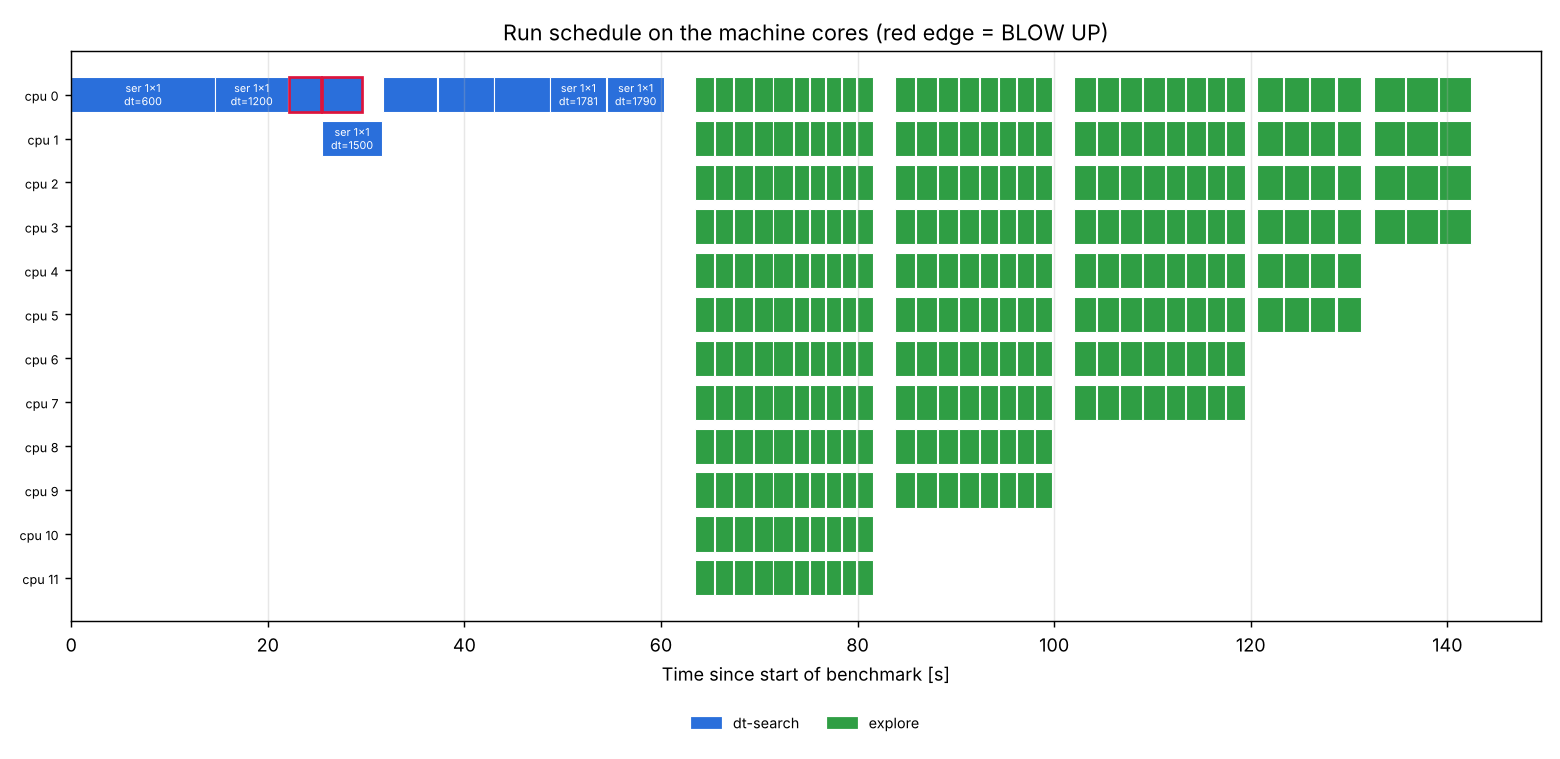
\includegraphics[width=\linewidth,height=0.55\textheight,keepaspectratio]{schedule.png}
\caption{Which run used which cores and when (red edge = BLOW UP).}
\end{figure}
\section{Methodology}
\begin{itemize}
\item Every run starts from the original \texttt{cppdefs.h}, \texttt{param.h} and \texttt{croco.in}. \texttt{cppdefs.h}: \texttt{OPENMP} or \texttt{MPI} switched inside the active configuration block (both undefined for the serial build); \texttt{param.h}: \texttt{NP\_XI}/\texttt{NP\_ETA} (MPI) or \texttt{NPP}/\texttt{NSUB\_X}/\texttt{NSUB\_E} (OpenMP); \texttt{croco.in}: \texttt{dt} and \texttt{NTIMES = ceil(30$\cdot$86400/dt)}. Output periods are rescaled to stay constant in seconds.
\item Case and grid are not assumed: the preprocessor directives of \texttt{cppdefs.h} are evaluated and then used to find the \texttt{parameter (LLm0=\ldots{}, MMm0=\ldots{}, N=\ldots{})} line of \texttt{param.h} that is actually compiled.
\item One executable per layout, compiled before the runs that use it, several at a time in sibling directories of \texttt{run\_dir}; changing dt does not recompile. Every run works in its own directory (\texttt{work/<run>}) with its own \texttt{croco.in}, inputs linked read-only, and is pinned to its own block of cores (\texttt{taskset}, \texttt{OMP\_PLACES}).
\item Measured time: wall-clock time from launch to process end. BLOW UP is detected in the log (\texttt{BLOW UP} or \texttt{NaN}); the run is killed after a grace period and runs with a larger dt are cancelled.
\item CFL barotropic = dt\_fast$\cdot$$\surd$(g$\cdot$h)$\cdot$$\surd$(1/dx$^2$+1/dy$^2$) (maximum over wet points, dt\_fast = dt/NDTFAST); CFL internal = dt$\cdot$c$_1$$\cdot$$\surd$(1/dx$^2$+1/dy$^2$) with an assumed c$_1$; CFL advective = dt$\cdot$max(|u|/dx + |v|/dy) from the history file.
\item Stability over the simulated period does not guarantee stability under stronger forcing: for production, keep a margin ($\approx$ 10--20 \% below the largest stable dt).
\end{itemize}
\section{Appendix: all runs}
{\scriptsize\rowcolors{2}{white}{zebra}
\begin{longtable}{llrcrrlrlrrp{0.16\linewidth}}
\caption{Every run of the benchmark, in order.}\\
\toprule
\textbf{Stage} & \textbf{Mode} & \textbf{Cores} & \textbf{Layout} & \textbf{dt} & \textbf{Rep} & \textbf{CPUs} & \textbf{Concurrent} & \textbf{Status} & \textbf{Time [s]} & \textbf{Sim. days} & \textbf{Notes} \\
\midrule
\endfirsthead
\toprule
\textbf{Stage} & \textbf{Mode} & \textbf{Cores} & \textbf{Layout} & \textbf{dt} & \textbf{Rep} & \textbf{CPUs} & \textbf{Concurrent} & \textbf{Status} & \textbf{Time [s]} & \textbf{Sim. days} & \textbf{Notes} \\
\midrule
\endhead
\bottomrule
\endfoot
dt-search & serial & 1 & 1$\times$1 & 600 & 0 & 0 & 0 & OK & 14.6 & 30.000 &  \\
dt-search & serial & 1 & 1$\times$1 & 1200 & 0 & 0 & 0 & OK & 7.4 & 30.000 &  \\
dt-search & serial & 1 & 1$\times$1 & 2400 & 0 & 0 & 0 & BLOWUP & 3.3 & 18.000 &  \\
dt-search & serial & 1 & 1$\times$1 & 1800 & 0 & 0 & 1 & BLOWUP & 4.1 & 18.000 &  \\
dt-search & serial & 1 & 1$\times$1 & 1500 & 0 & 1 & 1 & OK & 6.1 & 30.000 &  \\
dt-search & serial & 1 & 1$\times$1 & 1650 & 0 & 0 & 1 & OK & 5.6 & 30.002 &  \\
dt-search & serial & 1 & 1$\times$1 & 1725 & 0 & 0 & 1 & OK & 5.7 & 30.008 &  \\
dt-search & serial & 1 & 1$\times$1 & 1762 & 0 & 0 & 1 & OK & 5.6 & 30.019 &  \\
dt-search & serial & 1 & 1$\times$1 & 1781 & 0 & 0 & 1 & OK & 5.7 & 30.013 &  \\
dt-search & serial & 1 & 1$\times$1 & 1790 & 0 & 0 & 0 & OK & 5.8 & 30.020 &  \\
explore & openmp & 12 & 2$\times$6 & 1200 & 0 & 0-11 & 0 & OK & 1.9 & 30.000 &  \\
explore & openmp & 12 & 3$\times$4 & 1200 & 0 & 0-11 & 0 & OK & 1.9 & 30.000 &  \\
explore & openmp & 12 & 4$\times$3 & 1200 & 0 & 0-11 & 0 & OK & 1.9 & 30.000 &  \\
explore & openmp & 12 & 6$\times$2 & 1200 & 0 & 0-11 & 0 & OK & 1.9 & 30.000 &  \\
explore & openmp & 12 & 12$\times$1 & 1200 & 0 & 0-11 & 0 & OK & 1.9 & 30.000 &  \\
explore & mpi & 12 & 2$\times$6 & 1200 & 0 & 0-11 & 0 & OK & 1.6 & 30.000 &  \\
explore & mpi & 12 & 3$\times$4 & 1200 & 0 & 0-11 & 0 & OK & 1.5 & 30.000 &  \\
explore & mpi & 12 & 4$\times$3 & 1200 & 0 & 0-11 & 0 & OK & 1.5 & 30.000 &  \\
explore & mpi & 12 & 6$\times$2 & 1200 & 0 & 0-11 & 0 & OK & 1.5 & 30.000 &  \\
explore & mpi & 12 & 12$\times$1 & 1200 & 0 & 0-11 & 0 & OK & 1.6 & 30.000 &  \\
explore & openmp & 10 & 1$\times$10 & 1200 & 0 & 0-9 & 0 & OK & 2.1 & 30.000 &  \\
explore & openmp & 10 & 2$\times$5 & 1200 & 0 & 0-9 & 0 & OK & 2.1 & 30.000 &  \\
explore & openmp & 10 & 5$\times$2 & 1200 & 0 & 0-9 & 0 & OK & 2.0 & 30.000 &  \\
explore & openmp & 10 & 10$\times$1 & 1200 & 0 & 0-9 & 0 & OK & 2.1 & 30.000 &  \\
explore & mpi & 10 & 1$\times$10 & 1200 & 0 & 0-9 & 0 & OK & 1.8 & 30.000 &  \\
explore & mpi & 10 & 2$\times$5 & 1200 & 0 & 0-9 & 0 & OK & 1.7 & 30.000 &  \\
explore & mpi & 10 & 5$\times$2 & 1200 & 0 & 0-9 & 0 & OK & 1.7 & 30.000 &  \\
explore & mpi & 10 & 10$\times$1 & 1200 & 0 & 0-9 & 0 & OK & 1.8 & 30.000 &  \\
explore & openmp & 8 & 1$\times$8 & 1200 & 0 & 0-7 & 0 & OK & 2.2 & 30.000 &  \\
explore & openmp & 8 & 2$\times$4 & 1200 & 0 & 0-7 & 0 & OK & 2.3 & 30.000 &  \\
explore & openmp & 8 & 4$\times$2 & 1200 & 0 & 0-7 & 0 & OK & 2.2 & 30.000 &  \\
explore & openmp & 8 & 8$\times$1 & 1200 & 0 & 0-7 & 0 & OK & 2.2 & 30.000 &  \\
explore & mpi & 8 & 1$\times$8 & 1200 & 0 & 0-7 & 0 & OK & 1.9 & 30.000 &  \\
explore & mpi & 8 & 2$\times$4 & 1200 & 0 & 0-7 & 0 & OK & 1.9 & 30.000 &  \\
explore & mpi & 8 & 4$\times$2 & 1200 & 0 & 0-7 & 0 & OK & 1.8 & 30.000 &  \\
explore & mpi & 8 & 8$\times$1 & 1200 & 0 & 0-7 & 0 & OK & 1.9 & 30.000 &  \\
explore & openmp & 6 & 1$\times$6 & 1200 & 0 & 0-5 & 0 & OK & 2.6 & 30.000 &  \\
explore & openmp & 6 & 2$\times$3 & 1200 & 0 & 0-5 & 0 & OK & 2.5 & 30.000 &  \\
explore & openmp & 6 & 3$\times$2 & 1200 & 0 & 0-5 & 0 & OK & 2.6 & 30.000 &  \\
explore & openmp & 6 & 6$\times$1 & 1200 & 0 & 0-5 & 0 & OK & 2.5 & 30.000 &  \\
explore & openmp & 4 & 1$\times$4 & 1200 & 0 & 0-3 & 0 & OK & 3.2 & 30.000 &  \\
explore & openmp & 4 & 2$\times$2 & 1200 & 0 & 0-3 & 0 & OK & 3.2 & 30.000 &  \\
explore & openmp & 4 & 4$\times$1 & 1200 & 0 & 0-3 & 0 & OK & 3.2 & 30.000 &  \\
\end{longtable}}
\end{document}
